\section{Automated Doubling Experiments}
  \label{sec:technique}

  Our technique for performing automatic doubling experiments requires
  two parts.  The first is a rule for how to double the initial schema.
  The second is a rule for determining when a conclusion can be drawn
  from the experiment, and the experiment can be stopped. 

  \subsection{Doubling Schemas}
  \label{subsec:doubling}

  Determining worst case complexity by doubling experiment requires that
  the size of the input be doubled.  However, a relational database
  schema is a complex artifact with many features and
  interrelationships. This makes determining meaningful doubling rules a 
  non-trivial task.

  An example of semantic doubling is shown in
  Figure~\ref{fig:semanticconstraint}.


\begin{figure*}
\centering
  \centering
  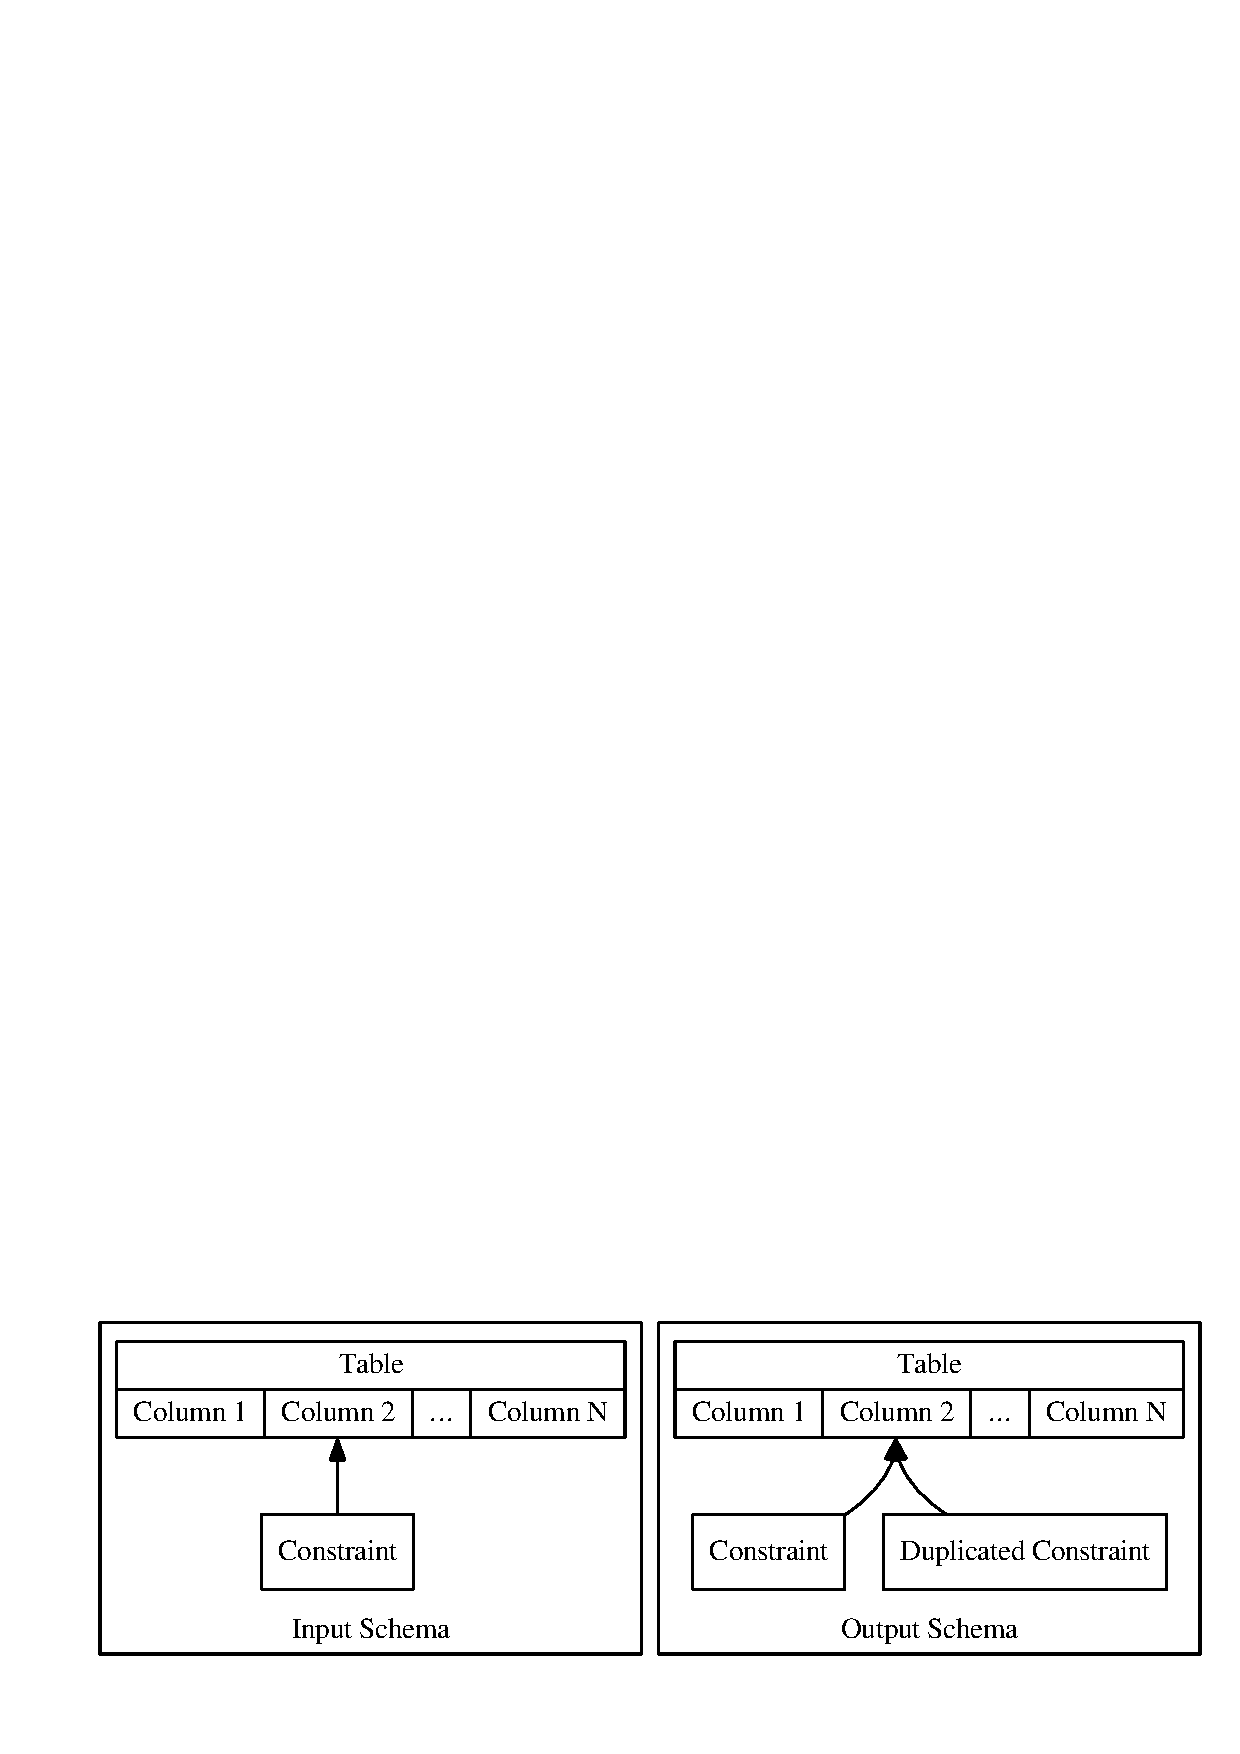
\includegraphics[width=.5\linewidth]{../diagrams/semanticconstraint.pdf}
  \caption{A table with a constraint before and after application of a semantic
  doubling rule.}
  \label{fig:semanticconstraint}
\end{figure*}


  \subsection{Automatic Experiment}
  \label{subsec:experiment}

To determine worst case complexity, an input $n$ is doubled until the 
ratio $f(2n) / f(n)$ converges to a stable value. To account for random
error, every time $n$ is doubled, $f(n)$ is recorded ten times, and the
median time is used for calculating the ratios.  We chose
median to minimize the effect of outliers. If mean is used instead, a
single abnormally long run could have a large effect on the result. The overall 
structure of the experiment is shown in Algorithm~\ref{alg:main}, and in
Figure~\ref{fig:doublingexp}.

\begin{figure*}
\centering
  \centering
  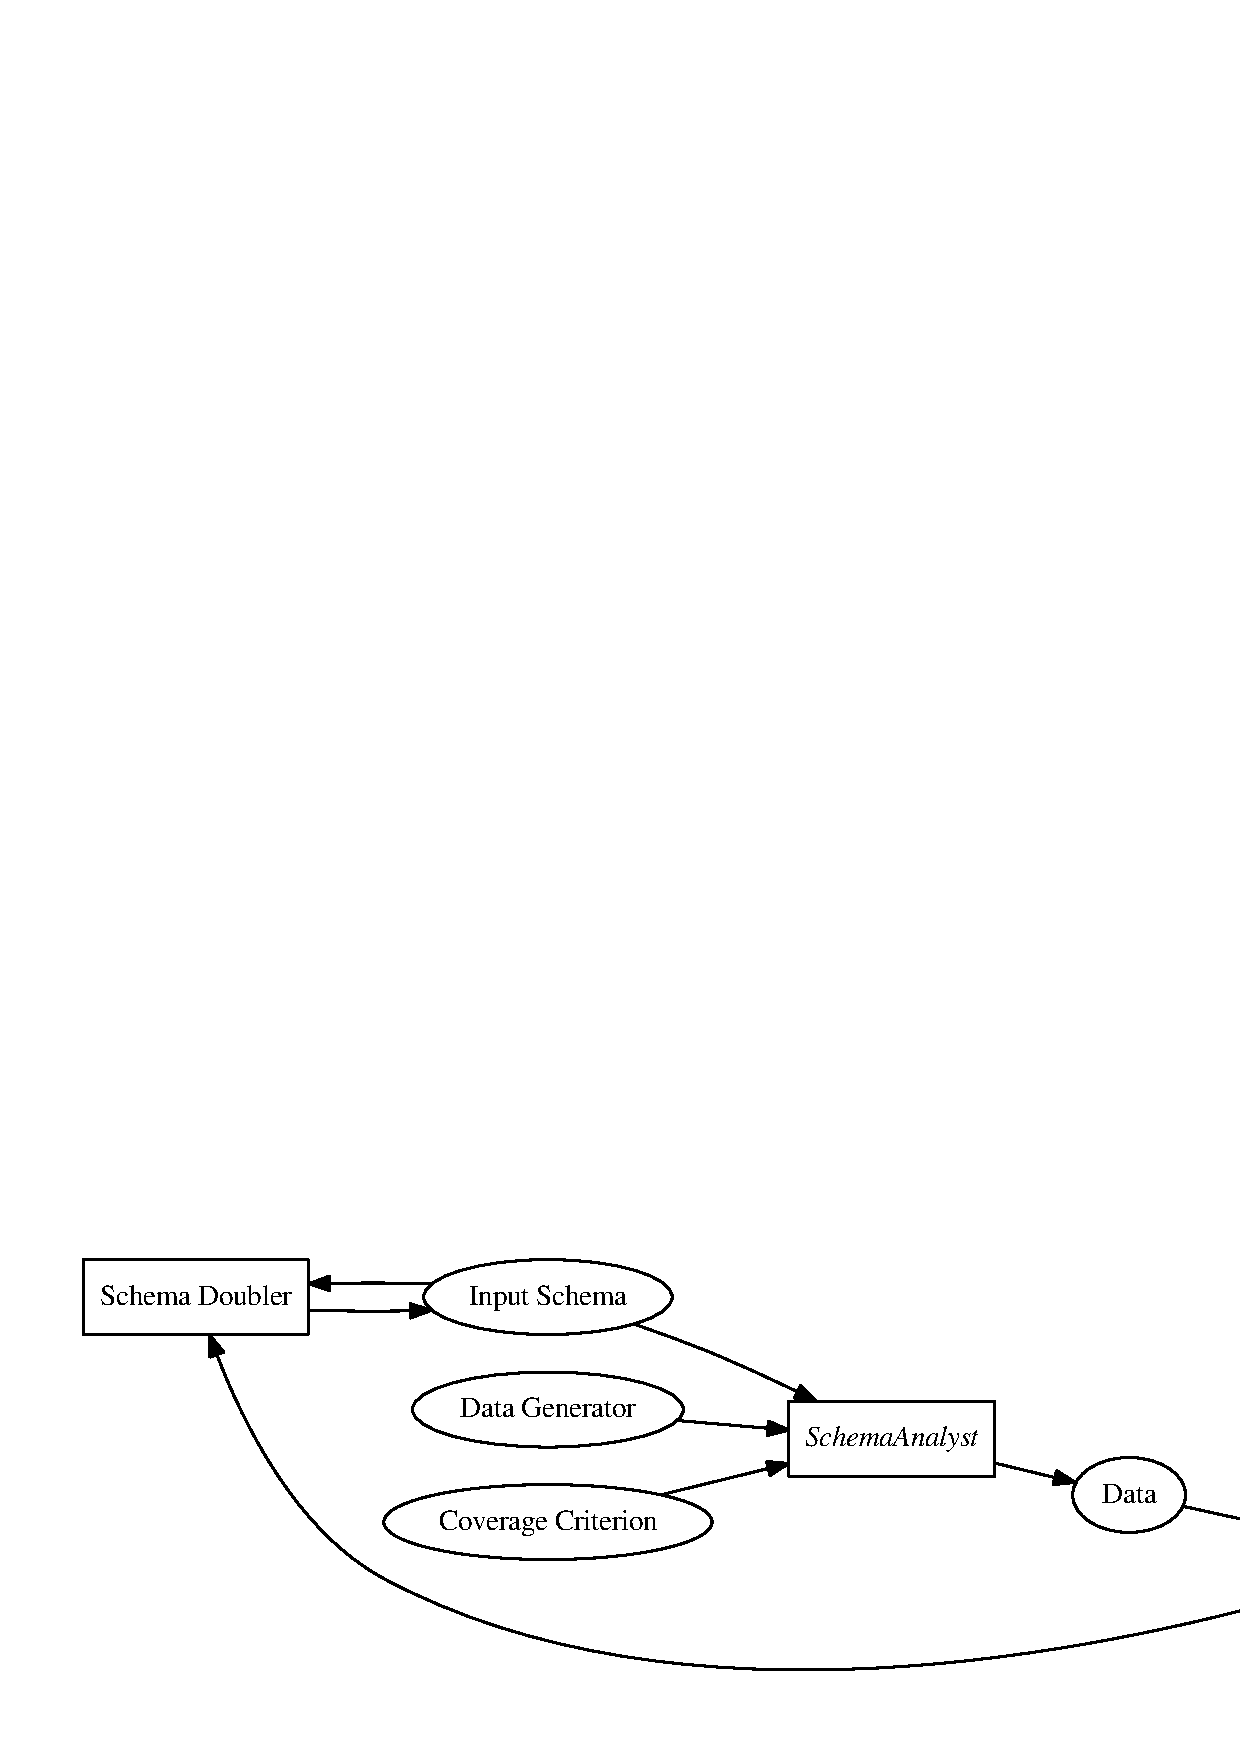
\includegraphics[width=.5\linewidth]{../diagrams/doublingexp.pdf}
  \caption{Technique for conducting automatic doubling experiments.}
  \label{fig:doublingexp}
\end{figure*}


This convergence checking is necessary because of the fact that worst-case
time is only apparent for large values of $n$. If too few doubles
are tried, then the experiment may terminate before $n$ reaches a value
where the true worst-case time complexity is apparent. At the same time,
for inefficient  algorithms, each additional double run incurs a substantial
time overhead. To conduct the testing efficiently, the experiment should
terminate as quickly as possible.

To test for convergence, the last four ratios are compared, and the
sum of differences between them is compared to a tolerance value. The
convergence algorithm is shown as Algorithm~\ref{alg:convergence}.
  
Another consequence of worst-case time only being apparent for large
$n$, is that a very small initial $n$ may appear to converge to $1$,
which indicates constant time. To prevent the
experiment from incorrectly terminating given a small starting $n$, we
require that a program under study display a ratio of $1$ for many
runs before judging that the ratio does in fact converge to $1$. Because 
$1$ signifies constant or logarithmic 
time, requiring these doubles does not significantly increase the time needed
to run the experiment, while providing assurance that a small ratio is not due
to an insufficiently small $n$. This rule is shown in 
Algorithm~\ref{alg:tuning}.

\begin{algorithm}[t]
    \caption{Run Doubling Experiment}
    \begin{algorithmic}
      \WHILE{Not Convergent || N not large enough}
      \FOR{$\mathit{trials}$}
        \STATE Run Test
        \ENDFOR
        \STATE Double Schema
        \ENDWHILE
    \end{algorithmic}
    \label{alg:main}
  \end{algorithm}

 \begin{algorithm}[t]
    \caption{Convergent}
    \begin{algorithmic}
      \STATE difference $= |(r_4 - r_3) + (r_3 -r_2) + (r_2 - r_1)|$
      \IF{difference $< \mathit{differanceTolerance}$}
      \RETURN Ratio is convergent
      \ELSE
      \RETURN Ratio is not convergent
      \ENDIF
    \end{algorithmic}
    \label{alg:convergence}
  \end{algorithm}

 \begin{algorithm}[t]
    \caption{N Large Enough}
    \begin{algorithmic}
      \IF{ratio $\approx 1$}
      \IF{number of doubles $< \mathit{doublesTolerance}$}
      \RETURN N is not large enough
      \ENDIF
      \ENDIF
      \RETURN N is large enough
    \end{algorithmic}
    \label{alg:tuning}
  \end{algorithm}
